\subsection{Methods}
For the first week, I implemented the random agent in \texttt{tic\_tac\_toe/agents/random\_agent.py}. I also implemented a decorator class in \texttt{tic\_tac\_toe/agents/timed\_agent.py} for timing and other statistics. Small changes were made in \texttt{main.py} and \texttt{tic\_tac\_toe/game.py} to record all the statistics needed for the report.

I have also begun working on the minimax agent, which I believe is fully functional. I may end up restructuring the code here in order to simplify the procedure for alpha-beta pruning in the following weeks.

\subsection{Results}
The following table shows the results of x/o wins and draws from 100 random games.
\[
    \begin{array}{|l|c|c|}
        \hline
        \textbf{x} & \textbf{o} & \textbf{draws}\\
        \hline
        55 & 31 & 14\\
        \hline
    \end{array}    
\]
As expected, the first agent (who plays x) generally has an advantage in a completely random game. This is likely due to the fact that the amount of x's is, at any given time, either equal to or 1 higher (a significant porportion in short games) than the amount of o's on the board.

The next plot shows the distribution of runtime per turn for random agents over the same 100 games.

\hspace*{.3in}
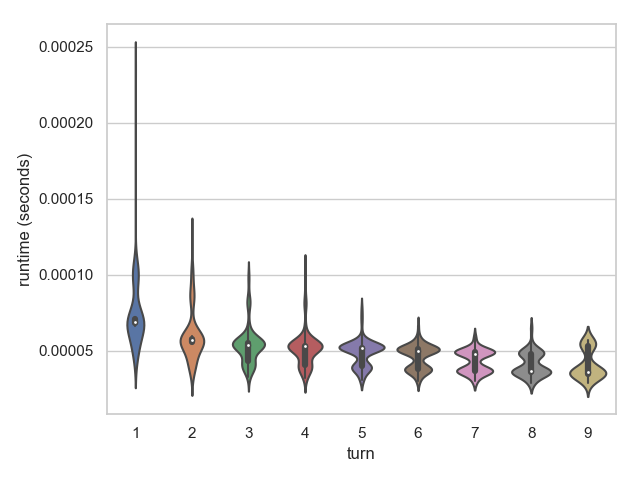
\includegraphics[scale=.7]{../../plots/random_random/runtime.png}

Runtime ranged from about 35 to 65 milliseconds per move. There is also a fairly steady descrease in runtime as the game progresses, which is likely due to the process of the \texttt{valid\_moves} method. This method constructs a \texttt{Move} object for each empty cell on the board, so less constructions will take place as the board fills up. The \texttt{random.choice} method itself completes in constant runtime.